\section{Histograms}

\ifCPy

\ifC
\cvfunc{CvHistogram}\label{CvHistogram}
Multi-dimensional histogram.

\begin{lstlisting}
typedef struct CvHistogram
{
    int     type;
    CvArr*  bins;
    float   thresh[CV_MAX_DIM][2]; /* for uniform histograms */
    float** thresh2; /* for non-uniform histograms */
    CvMatND mat; /* embedded matrix header for array histograms */
}
CvHistogram;
\end{lstlisting}
\fi

\cvCPyFunc{CalcBackProject}
Calculates the back projection.

\cvdefC{
void cvCalcBackProject( \par IplImage** image,\par CvArr* back\_project,\par const CvHistogram* hist );
}\cvdefPy{CalcBackProject(image,back\_project,hist)-> None}

\begin{description}
\cvarg{image}{Source images (though you may pass CvMat** as well)}
\cvarg{back\_project}{Destination back projection image of the same type as the source images}
\cvarg{hist}{Histogram}
\end{description}

The function calculates the back project of the histogram. For each tuple of pixels at the same position of all input single-channel images the function puts the value of the histogram bin, corresponding to the tuple in the destination image. In terms of statistics, the value of each output image pixel is the probability of the observed tuple given the distribution (histogram). For example, to find a red object in the picture, one may do the following:

\begin{enumerate}
 \item Calculate a hue histogram for the red object assuming the image contains only this object. The histogram is likely to have a strong maximum, corresponding to red color.
 \item Calculate back projection of a hue plane of input image where the object is searched, using the histogram. Threshold the image.
 \item Find connected components in the resulting picture and choose the right component using some additional criteria, for example, the largest connected component.
\end{enumerate}

That is the approximate algorithm of Camshift color object tracker, except for the 3rd step, instead of which CAMSHIFT algorithm is used to locate the object on the back projection given the previous object position.

\cvCPyFunc{CalcBackProjectPatch}
Locates a template within an image by using a histogram comparison.

\cvdefC{
void cvCalcBackProjectPatch( \par IplImage** image,\par CvArr* dst,\par CvSize patch\_size,\par CvHistogram* hist,\par int method,\par float factor );
}\cvdefPy{CalcBackProjectPatch(images,dst,patch\_size,hist,method,factor)-> None}

\begin{description}
\cvarg{image}{Source images (though, you may pass CvMat** as well)}
\cvarg{dst}{Destination image}
\cvarg{patch\_size}{Size of the patch slid though the source image}
\cvarg{hist}{Histogram}
\cvarg{method}{Compasion method, passed to \cvCPyCross{CompareHist} (see description of that function)}
\cvarg{factor}{Normalization factor for histograms, will affect the normalization scale of the destination image, pass 1 if unsure}
\end{description}

The function calculates the back projection by comparing histograms of the source image patches with the given histogram. Taking measurement results from some image at each location over ROI creates an array \texttt{image}. These results might be one or more of hue, \texttt{x} derivative, \texttt{y} derivative, Laplacian filter, oriented Gabor filter, etc. Each measurement output is collected into its own separate image. The \texttt{image} image array is a collection of these measurement images. A multi-dimensional histogram \texttt{hist} is constructed by sampling from the \texttt{image} image array. The final histogram is normalized. The \texttt{hist} histogram has as many dimensions as the number of elements in \texttt{image} array.

Each new image is measured and then converted into an \texttt{image} image array over a chosen ROI. Histograms are taken from this \texttt{image} image in an area covered by a "patch" with an anchor at center as shown in the picture below. The histogram is normalized using the parameter \texttt{norm\_factor} so that it may be compared with \texttt{hist}. The calculated histogram is compared to the model histogram; \texttt{hist} uses The function \texttt{cvCompareHist} with the comparison method=\texttt{method}). The resulting output is placed at the location corresponding to the patch anchor in the probability image \texttt{dst}. This process is repeated as the patch is slid over the ROI. Iterative histogram update by subtracting trailing pixels covered by the patch and adding newly covered pixels to the histogram can save a lot of operations, though it is not implemented yet.

Back Project Calculation by Patches

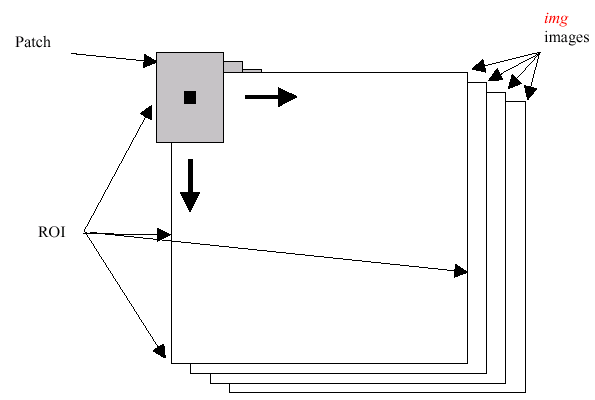
\includegraphics[width=0.5\textwidth]{pics/backprojectpatch.png}

\cvCPyFunc{CalcHist}
Calculates the histogram of image(s).

\cvdefC{
void cvCalcHist( \par IplImage** image,\par CvHistogram* hist,\par int accumulate=0,\par const CvArr* mask=NULL );
}
\cvdefPy{CalcHist(image,hist,accumulate=0,mask=NULL)-> None}

\begin{description}
\cvarg{image}{Source images (though you may pass CvMat** as well)}
\cvarg{hist}{Pointer to the histogram}
\cvarg{accumulate}{Accumulation flag. If it is set, the histogram is not cleared in the beginning. This feature allows user to compute a single histogram from several images, or to update the histogram online}
\cvarg{mask}{The operation mask, determines what pixels of the source images are counted}
\end{description}

The function calculates the histogram of one or more
single-channel images. The elements of a tuple that is used to increment
a histogram bin are taken at the same location from the corresponding
input images.

% ===== Sample. Calculating and displaying 2D Hue-Saturation histogram of a color image =====
\begin{lstlisting}
#include <cv.h>
#include <highgui.h>

int main( int argc, char** argv )
{
    IplImage* src;
    if( argc == 2 && (src=cvLoadImage(argv[1], 1))!= 0)
    {
        IplImage* h_plane = cvCreateImage( cvGetSize(src), 8, 1 );
        IplImage* s_plane = cvCreateImage( cvGetSize(src), 8, 1 );
        IplImage* v_plane = cvCreateImage( cvGetSize(src), 8, 1 );
        IplImage* planes[] = { h_plane, s_plane };
        IplImage* hsv = cvCreateImage( cvGetSize(src), 8, 3 );
        int h_bins = 30, s_bins = 32;
        int hist_size[] = {h_bins, s_bins};
        /* hue varies from 0 (~0 deg red) to 180 (~360 deg red again) */
        float h_ranges[] = { 0, 180 };
        /* saturation varies from 0 (black-gray-white) to
           255 (pure spectrum color) */
        float s_ranges[] = { 0, 255 };
        float* ranges[] = { h_ranges, s_ranges };
        int scale = 10;
        IplImage* hist_img =
            cvCreateImage( cvSize(h_bins*scale,s_bins*scale), 8, 3 );
        CvHistogram* hist;
        float max_value = 0;
        int h, s;

        cvCvtColor( src, hsv, CV_BGR2HSV );
        cvCvtPixToPlane( hsv, h_plane, s_plane, v_plane, 0 );
        hist = cvCreateHist( 2, hist_size, CV_HIST_ARRAY, ranges, 1 );
        cvCalcHist( planes, hist, 0, 0 );
        cvGetMinMaxHistValue( hist, 0, &max_value, 0, 0 );
        cvZero( hist_img );

        for( h = 0; h < h_bins; h++ )
        {
            for( s = 0; s < s_bins; s++ )
            {
                float bin_val = cvQueryHistValue_2D( hist, h, s );
                int intensity = cvRound(bin_val*255/max_value);
                cvRectangle( hist_img, cvPoint( h*scale, s*scale ),
                             cvPoint( (h+1)*scale - 1, (s+1)*scale - 1),
                             CV_RGB(intensity,intensity,intensity),
                             CV_FILLED );
            }
        }

        cvNamedWindow( "Source", 1 );
        cvShowImage( "Source", src );

        cvNamedWindow( "H-S Histogram", 1 );
        cvShowImage( "H-S Histogram", hist_img );

        cvWaitKey(0);
    }
}
\end{lstlisting}

\cvCPyFunc{CalcProbDensity}
Divides one histogram by another.

\cvdefC{
void  cvCalcProbDensity( \par const CvHistogram* hist1,\par const CvHistogram* hist2,\par CvHistogram* dst\_hist,\par double scale=255 );
}\cvdefPy{CalcProbDensity(hist1,hist2,dst\_hst,scale=255)-> None}

\begin{description}
\cvarg{hist1}{first histogram (the divisor)}
\cvarg{hist2}{second histogram}
\cvarg{dst\_hist}{destination histogram}
\cvarg{scale}{scale factor for the destination histogram}
\end{description}

The function calculates the object probability density from the two histograms as:

\[
\texttt{dist\_hist}(I)=
\forkthree
{0}{if $\texttt{hist1}(I)=0$}
{\texttt{scale}}{if $\texttt{hist1}(I) \ne 0$ and $\texttt{hist2}(I) > \texttt{hist1}(I)$}
{\frac{\texttt{hist2}(I) \cdot \texttt{scale}}{\texttt{hist1}(I)}}{if $\texttt{hist1}(I) \ne 0$ and $\texttt{hist2}(I) \le \texttt{hist1}(I)$}
\]

So the destination histogram bins are within less than \texttt{scale}.

\cvCPyFunc{ClearHist}
Clears the histogram.

\cvdefC{
void cvClearHist( CvHistogram* hist );
}\cvdefPy{ClearHist(hist)-> None}

\begin{description}
\cvarg{hist}{Histogram}
\end{description}

The function sets all of the histogram bins to 0 in the case of a dense histogram and removes all histogram bins in the case of a sparse array.

\cvCPyFunc{CompareHist}
Compares two dense histograms.

\cvdefC{
double cvCompareHist( \par const CvHistogram* hist1,\par const CvHistogram* hist2,\par int method );
}\cvdefPy{CompareHist(hist1,hist2,method)->float}

\begin{description}
\cvarg{hist1}{The first dense histogram}
\cvarg{hist2}{The second dense histogram}
\cvarg{method}{Comparison method, one of the following:
\begin{description}
  \cvarg{CV\_COMP\_CORREL}{Correlation}
  \cvarg{CV\_COMP\_CHISQR}{Chi-Square}
  \cvarg{CV\_COMP\_INTERSECT}{Intersection}
  \cvarg{CV\_COMP\_BHATTACHARYYA}{Bhattacharyya distance}
\end{description}}
\end{description}

The function compares two dense histograms using the specified method ($H_1$ denotes the first histogram, $H_2$ the second):

\begin{description}
\item[Correlation (method=CV\_COMP\_CORREL)]
\[
d(H_1,H_2) = \frac
{\sum_I (H'_1(I) \cdot H'_2(I))}
{\sqrt{\sum_I(H'_1(I)^2) \cdot \sum_I(H'_2(I)^2)}}
\]
where
\[
H'_k(I) = \frac{H_k(I) - 1}{N \cdot \sum_J H_k(J)}
\]
where N is the number of histogram bins.

\item[Chi-Square (method=CV\_COMP\_CHISQR)]
\[ d(H_1,H_2) = \sum_I \frac{(H_1(I)-H_2(I))^2}{H_1(I)+H_2(I)} \]

\item[Intersection (method=CV\_COMP\_INTERSECT)]
\[ d(H_1,H_2) = \sum_I \min (H_1(I), H_2(I)) \]

\item[Bhattacharyya distance (method=CV\_COMP\_BHATTACHARYYA)]
\[ d(H_1,H_2) = \sqrt{1 - \sum_I \frac{\sqrt{H_1(I) \cdot H_2(I)}}{ \sqrt { \sum_I H_1(I) \cdot \sum_I H_2(I) }}} \]

\end{description}

The function returns $d(H_1, H_2)$.

Note: the method \texttt{CV\_COMP\_BHATTACHARYYA} only works with normalized histograms.

To compare a sparse histogram or more general sparse configurations of weighted points, consider using the \cvCPyCross{CalcEMD2} function.

\ifC
\cvCPyFunc{CopyHist}
Copies a histogram.

\cvdefC{
void cvCopyHist( const CvHistogram* src, CvHistogram** dst );
}

\begin{description}
\cvarg{src}{Source histogram}
\cvarg{dst}{Pointer to destination histogram}
\end{description}

The function makes a copy of the histogram. If the
second histogram pointer \texttt{*dst} is NULL, a new histogram of the
same size as \texttt{src} is created. Otherwise, both histograms must
have equal types and sizes. Then the function copies the source histogram's
bin values to the destination histogram and sets the same bin value ranges
as in \texttt{src}.

\fi

\cvCPyFunc{CreateHist}
Creates a histogram.

\cvdefC{
CvHistogram* cvCreateHist(\par int dims,\par int* sizes,\par int type,\par float** ranges=NULL,\par int uniform=1 );
}\cvdefPy{CreateHist(dims, type, ranges, uniform = 1) -> hist}

\begin{description}
\cvC{\cvarg{dims}{Number of histogram dimensions}
\cvarg{sizes}{Array of the histogram dimension sizes}}
\cvPy{\cvarg{dims}{for an N-dimensional histogram, list of length N giving the size of each dimension}}
\cvarg{type}{Histogram representation format: \texttt{CV\_HIST\_ARRAY} means that the histogram data is represented as a multi-dimensional dense array CvMatND; \texttt{CV\_HIST\_SPARSE} means that histogram data is represented as a multi-dimensional sparse array CvSparseMat}
\cvarg{ranges}{Array of ranges for the histogram bins. Its meaning depends on the \texttt{uniform} parameter value. The ranges are used for when the histogram is calculated or backprojected to determine which histogram bin corresponds to which value/tuple of values from the input image(s)}
\cvarg{uniform}{Uniformity flag; if not 0, the histogram has evenly
spaced bins and for every $0<=i<cDims$ \texttt{ranges[i]}
is an array of two numbers: lower and upper boundaries for the i-th
histogram dimension.
The whole range [lower,upper] is then split
into \texttt{dims[i]} equal parts to determine the \texttt{i-th} input
tuple value ranges for every histogram bin. And if \texttt{uniform=0},
then \texttt{i-th} element of \texttt{ranges} array contains
\texttt{dims[i]+1} elements:
$\texttt{lower}_0, \texttt{upper}_0, 
\texttt{lower}_1, \texttt{upper}_1 = \texttt{lower}_2,
...
\texttt{upper}_{dims[i]-1} $
where
$\texttt{lower}_j$ and $\texttt{upper}_j$
are lower and upper
boundaries of \texttt{i-th} input tuple value for \texttt{j-th}
bin, respectively. In either case, the input values that are beyond
the specified range for a histogram bin are not counted by
\cvCPyCross{CalcHist} and filled with 0 by \cvCPyCross{CalcBackProject}}
\end{description}

The function creates a histogram of the specified
size and returns a pointer to the created histogram. If the array
\texttt{ranges} is 0, the histogram bin ranges must be specified later
via the function \cvCPyCross{SetHistBinRanges}. Though \cvCPyCross{CalcHist}
and \cvCPyCross{CalcBackProject} may process 8-bit images without setting
bin ranges, they assume thy are equally spaced in 0 to 255 bins.

\ifC % {
\cvCPyFunc{GetHistValue*D}
Returns a pointer to the histogram bin.

\begin{lstlisting}
#define cvGetHistValue_1D( hist, idx0 ) 
    ((float*)(cvPtr1D( (hist)->bins, (idx0), 0 ))
#define cvGetHistValue_2D( hist, idx0, idx1 ) 
    ((float*)(cvPtr2D( (hist)->bins, (idx0), (idx1), 0 )))
#define cvGetHistValue_3D( hist, idx0, idx1, idx2 ) 
    ((float*)(cvPtr3D( (hist)->bins, (idx0), (idx1), (idx2), 0 )))
#define cvGetHistValue_nD( hist, idx ) 
    ((float*)(cvPtrND( (hist)->bins, (idx), 0 )))
\end{lstlisting}

\begin{description}
\cvarg{hist}{Histogram}
\cvarg{idx0, idx1, idx2, idx3}{Indices of the bin}
\cvarg{idx}{Array of indices}
\end{description}

The macros \texttt{GetHistValue} return a pointer to the specified bin of the 1D, 2D, 3D or N-D histogram. In the case of a sparse histogram the function creates a new bin and sets it to 0, unless it exists already.
\fi % }

\cvCPyFunc{GetMinMaxHistValue}
Finds the minimum and maximum histogram bins.

\cvdefC{
void cvGetMinMaxHistValue( \par const CvHistogram* hist,\par float* min\_value,\par float* max\_value,\par int* min\_idx=NULL,\par int* max\_idx=NULL );

}
\cvdefPy{GetMinMaxHistValue(hist)-> (min\_val,max\_val,min\_loc,max\_loc)}

\begin{description}
\cvarg{hist}{Histogram}
\cvarg{min\_value}{Pointer to the minimum value of the histogram}
\cvarg{max\_value}{Pointer to the maximum value of the histogram}
\cvarg{min\_idx}{Pointer to the array of coordinates for the minimum}
\cvarg{max\_idx}{Pointer to the array of coordinates for the maximum}
\end{description}

The function finds the minimum and
maximum histogram bins and their positions. All of output arguments are
optional. Among several extremas with the same value the ones with the
minimum index (in lexicographical order) are returned. In the case of several maximums
or minimums, the earliest in lexicographical order (extrema locations)
is returned.

\ifC % {
\cvCPyFunc{MakeHistHeaderForArray}
Makes a histogram out of an array.

\cvdefC{
CvHistogram*  cvMakeHistHeaderForArray( \par int dims,\par int* sizes,\par CvHistogram* hist,\par float* data,\par float** ranges=NULL,\par int uniform=1 );
}

\begin{description}
\cvarg{dims}{Number of histogram dimensions}
\cvarg{sizes}{Array of the histogram dimension sizes}
\cvarg{hist}{The histogram header initialized by the function}
\cvarg{data}{Array that will be used to store histogram bins}
\cvarg{ranges}{Histogram bin ranges, see \cvCPyCross{CreateHist}}
\cvarg{uniform}{Uniformity flag, see \cvCPyCross{CreateHist}}
\end{description}

The function initializes the histogram, whose header and bins are allocated by th user. \cvCPyCross{ReleaseHist} does not need to be called afterwards. Only dense histograms can be initialized this way. The function returns \texttt{hist}.
\fi % }

\cvCPyFunc{NormalizeHist}
Normalizes the histogram.

\cvdefC{
void cvNormalizeHist( CvHistogram* hist, double factor );
}\cvdefPy{NormalizeHist(hist,factor)-> None}

\begin{description}
\cvarg{hist}{Pointer to the histogram}
\cvarg{factor}{Normalization factor}
\end{description}

The function normalizes the histogram bins by scaling them, such that the sum of the bins becomes equal to \texttt{factor}.

\cvCPyFunc{QueryHistValue*D}
Queries the value of the histogram bin.

\begin{lstlisting}
#define cvQueryHistValue\_1D( hist, idx0 ) \
    cvGetReal1D( (hist)->bins, (idx0) )
#define cvQueryHistValue\_2D( hist, idx0, idx1 ) \
    cvGetReal2D( (hist)->bins, (idx0), (idx1) )
#define cvQueryHistValue\_3D( hist, idx0, idx1, idx2 ) \
    cvGetReal3D( (hist)->bins, (idx0), (idx1), (idx2) )
#define cvQueryHistValue\_nD( hist, idx ) \
    cvGetRealND( (hist)->bins, (idx) )
\end{lstlisting}

\begin{description}
\cvarg{hist}{Histogram}
\cvarg{idx0, idx1, idx2, idx3}{Indices of the bin}
\cvarg{idx}{Array of indices}
\end{description}

The macros return the value of the specified bin of the 1D, 2D, 3D or N-D histogram. In the case of a sparse histogram the function returns 0, if the bin is not present in the histogram no new bin is created.

\ifC
\cvCPyFunc{ReleaseHist}
Releases the histogram.

\cvdefC{
void cvReleaseHist( CvHistogram** hist );
}

\begin{description}
\cvarg{hist}{Double pointer to the released histogram}
\end{description}

The function releases the histogram (header and the data). The pointer to the histogram is cleared by the function. If \texttt{*hist} pointer is already \texttt{NULL}, the function does nothing.

\cvCPyFunc{SetHistBinRanges}
Sets the bounds of the histogram bins.

\cvdefC{
void cvSetHistBinRanges( \par CvHistogram* hist,\par float** ranges,\par int uniform=1 );
}

\begin{description}
\cvarg{hist}{Histogram}
\cvarg{ranges}{Array of bin ranges arrays, see \cvCPyCross{CreateHist}}
\cvarg{uniform}{Uniformity flag, see \cvCPyCross{CreateHist}}
\end{description}

The function is a stand-alone function for setting bin ranges in the histogram. For a more detailed description of the parameters \texttt{ranges} and \texttt{uniform} see the \cvCPyCross{CalcHist} function, that can initialize the ranges as well. Ranges for the histogram bins must be set before the histogram is calculated or the backproject of the histogram is calculated.

\fi

\cvCPyFunc{ThreshHist}
Thresholds the histogram.

\cvdefC{
void cvThreshHist( CvHistogram* hist, double threshold );
}
\cvdefPy{ThreshHist(hist,threshold)-> None}

\begin{description}
\cvarg{hist}{Pointer to the histogram}
\cvarg{threshold}{Threshold level}
\end{description}

The function clears histogram bins that are below the specified threshold.

\fi

\ifCpp

\cvCppFunc{calcHist}
Calculates histogram of a set of arrays

\cvdefCpp{void calcHist( const Mat* arrays, int narrays,\par
               const int* channels, const Mat\& mask,\par
               MatND\& hist, int dims, const int* histSize,\par
               const float** ranges, bool uniform=true,\par
               bool accumulate=false );\newline
void calcHist( const Mat* arrays, int narrays,\par
               const int* channels, const Mat\& mask,\par
               SparseMat\& hist, int dims, const int* histSize,\par
               const float** ranges, bool uniform=true,\par
               bool accumulate=false );}
\begin{description}
\cvarg{arrays}{Source arrays. They all should have the same depth, \texttt{CV\_8U} or \texttt{CV\_32F}, and the same size. Each of them can have an arbitrary number of channels}
\cvarg{narrays}{The number of source arrays}
\cvarg{channels}{The list of \texttt{dims} channels that are used to compute the histogram. The first array channels are numerated from 0 to \texttt{arrays[0].channels()-1}, the second array channels are counted from \texttt{arrays[0].channels()} to \texttt{arrays[0].channels() + arrays[1].channels()-1} etc.}
\cvarg{mask}{The optional mask. If the matrix is not empty, it must be 8-bit array of the same size as \texttt{arrays[i]}. The non-zero mask elements mark the array elements that are counted in the histogram}
\cvarg{hist}{The output histogram, a dense or sparse \texttt{dims}-dimensional array}
\cvarg{dims}{The histogram dimensionality; must be positive and not greater than \texttt{CV\_MAX\_DIMS}(=32 in the current OpenCV version)}
\cvarg{histSize}{The array of histogram sizes in each dimension}
\cvarg{ranges}{The array of \texttt{dims} arrays of the histogram bin boundaries in each dimension. When the histogram is uniform (\texttt{uniform}=true), then for each dimension \texttt{i} it's enough to specify the lower (inclusive) boundary $L_0$ of the 0-th histogram bin and the upper (exclusive) boundary $U_{\texttt{histSize}[i]-1}$ for the last histogram bin \texttt{histSize[i]-1}. That is, in the case of uniform histogram each of \texttt{ranges[i]} is an array of 2 elements. When the histogram is not uniform (\texttt{uniform=false}), then each of \texttt{ranges[i]} contains \texttt{histSize[i]+1} elements: $L_0, U_0=L_1, U_1=L_2, ..., U_{\texttt{histSize[i]}-2}=L_{\texttt{histSize[i]}-1}, U_{\texttt{histSize[i]}-1}$. The array elements, which are not between $L_0$ and $U_{\texttt{histSize[i]}-1}$, are not counted in the histogram}
\cvarg{uniform}{Indicates whether the histogram is uniform or not, see above}
\cvarg{accumulate}{Accumulation flag. If it is set, the histogram is not cleared in the beginning (when it is allocated). This feature allows user to compute a single histogram from several sets of arrays, or to update the histogram in time}
\end{description}

The functions \texttt{calcHist} calculate the histogram of one or more
arrays. The elements of a tuple that is used to increment
a histogram bin are taken at the same location from the corresponding
input arrays. The sample below shows how to compute 2D Hue-Saturation histogram for a color imag

\begin{lstlisting}
#include <cv.h>
#include <highgui.h>

using namespace cv;

int main( int argc, char** argv )
{
    Mat src;
    if( argc != 2 || !(src=imread(argv[1], 1)).data )
        return -1;

    Mat hsv;
    cvtColor(src, hsv, CV_BGR2HSV);

    // let's quantize the hue to 30 levels
    // and the saturation to 32 levels
    int hbins = 30, sbins = 32;
    int histSize[] = {hbins, sbins};
    // hue varies from 0 to 179, see cvtColor
    float hranges[] = { 0, 180 };
    // saturation varies from 0 (black-gray-white) to
    // 255 (pure spectrum color)
    float sranges[] = { 0, 256 };
    float* ranges[] = { hranges, sranges };
    MatND hist;
    // we compute the histogram from the 0-th and 1-st channels
    int channels[] = {0, 1};
    
    calcHist( &hsv, 1, channels, Mat(), // do not use mask
        hist, 2, histSize, ranges,
        true, // the histogram is uniform
        false );
    double maxVal=0;
    minMaxLoc(hist, 0, &maxVal, 0, 0);
    
    int scale = 10;
    Mat histImg = Mat::zeros(sbins*scale, hbins*10, CV_8UC3);        

    for( int h = 0; h < hbins; h++ )
        for( int s = 0; s < sbins; s++ )
        {
            float binVal = hist.at<float>(h, s);
            int intensity = cvRound(binVal*255/maxValue);
            cvRectangle( histImg, Point(h*scale, s*scale),
                         Point( (h+1)*scale - 1, (s+1)*scale - 1),
                         Scalar::all(intensity),
                         CV_FILLED );
        }

    namedWindow( "Source", 1 );
    imshow( "Source", src );

    namedWindow( "H-S Histogram", 1 );
    imshow( "H-S Histogram", histImg );

    waitKey();
}
\end{lstlisting}


\cvCppFunc{calcBackProject}
Calculates the back projection of a histogram.

\cvdefCpp{void calcBackProject( const Mat* arrays, int narrays,\par
                      const int* channels, const MatND\& hist,\par
                      Mat\& backProject, const float** ranges,\par
                      double scale=1, bool uniform=true );\newline
void calcBackProject( const Mat* arrays, int narrays,\par
                      const int* channels, const SparseMat\& hist,\par
                      Mat\& backProject, const float** ranges,\par
                      double scale=1, bool uniform=true );}
\begin{description}
\cvarg{arrays}{Source arrays. They all should have the same depth, \texttt{CV\_8U} or \texttt{CV\_32F}, and the same size. Each of them can have an arbitrary number of channels}
\cvarg{narrays}{The number of source arrays}
\cvarg{channels}{The list of channels that are used to compute the back projection. The number of channels must match the histogram dimensionality. The first array channels are numerated from 0 to \texttt{arrays[0].channels()-1}, the second array channels are counted from \texttt{arrays[0].channels()} to \texttt{arrays[0].channels() + arrays[1].channels()-1} etc.}
\cvarg{hist}{The input histogram, a dense or sparse}
\cvarg{backProject}{Destination back projection aray; will be a single-channel array of the same size and the same depth as \texttt{arrays[0]}}
\cvarg{ranges}{The array of arrays of the histogram bin boundaries in each dimension. See \cvCppCross{calcHist}}
\cvarg{scale}{The optional scale factor for the output back projection}
\cvarg{uniform}{Indicates whether the histogram is uniform or not, see above}
\end{description}

The functions \texttt{calcBackProject} calculate the back project of the histogram. That is, similarly to \texttt{calcHist}, at each location \texttt{(x, y)} the function collects the values from the selected channels in the input images and finds the corresponding histogram bin. But instead of incrementing it, the function reads the bin value, scales it by \texttt{scale} and stores in \texttt{backProject(x,y)}. In terms of statistics, the function computes probability of each element value in respect with the empirical probability distribution represented by the histogram. Here is how, for example, you can find and track a bright-colored object in a scene:

\begin{enumerate}
 \item Before the tracking, show the object to the camera such that covers almost the whole frame. Calculate a hue histogram. The histogram will likely have a strong maximums, corresponding to the dominant colors in the object.
 \item During the tracking, calculate back projection of a hue plane of each input video frame using that pre-computed histogram. Threshold the back projection to suppress weak colors. It may also have sense to suppress pixels with non sufficient color saturation and too dark or too bright pixels.
 \item Find connected components in the resulting picture and choose, for example, the largest component.
\end{enumerate}

That is the approximate algorithm of \cvCppCross{CAMShift} color object tracker.

See also: \cvCppCross{calcHist}

\cvCppFunc{compareHist}
Compares two histograms

\cvdefCpp{double compareHist( const MatND\& H1, const MatND\& H2, int method );\newline
double compareHist( const SparseMat\& H1, \par const SparseMat\& H2, int method );}
\begin{description}
\cvarg{H1}{The first compared histogram}
\cvarg{H2}{The second compared histogram of the same size as \texttt{H1}}
\cvarg{method}{The comparison method, one of the following:
\begin{description}
  \cvarg{CV\_COMP\_CORREL}{Correlation}
  \cvarg{CV\_COMP\_CHISQR}{Chi-Square}
  \cvarg{CV\_COMP\_INTERSECT}{Intersection}
  \cvarg{CV\_COMP\_BHATTACHARYYA}{Bhattacharyya distance}
\end{description}}
\end{description}

The functions \texttt{compareHist} compare two dense or two sparse histograms using the specified method:

\begin{description}
\item[Correlation (method=CV\_COMP\_CORREL)]
\[
d(H_1,H_2) = \frac
{\sum_I (H_1(I) - \bar{H_1}) (H_2(I) - \bar{H_2})}
{\sqrt{\sum_I(H_1(I) - \bar{H_1})^2 \sum_I(H_2(I) - \bar{H_2})^2}}
\]
where
\[
\bar{H_k} = \frac{1}{N} \sum_J H_k(J)
\]
and $N$ is the total number of histogram bins.

\item[Chi-Square (method=CV\_COMP\_CHISQR)]
\[ d(H_1,H_2) = \sum_I \frac{\left(H_1(I)-H_2(I)\right)^2}{H_1(I)+H_2(I)} \]

\item[Intersection (method=CV\_COMP\_INTERSECT)]
\[ d(H_1,H_2) = \sum_I \min (H_1(I), H_2(I)) \]

\item[Bhattacharyya distance (method=CV\_COMP\_BHATTACHARYYA)]
\[ d(H_1,H_2) = \sqrt{1 - \frac{1}{\sqrt{\bar{H_1} \bar{H_2} N^2}} \sum_I \sqrt{H_1(I) \cdot H_2(I)}} \]

\end{description}

The function returns $d(H_1, H_2)$.

While the function works well with 1-, 2-, 3-dimensional dense histograms, it may not be suitable for high-dimensional sparse histograms, where, because of aliasing and sampling problems the coordinates of non-zero histogram bins can slightly shift. To compare such histograms or more general sparse configurations of weighted points, consider using the \cvCppCross{calcEMD} function.

\cvCppFunc{equalizeHist}
Equalizes the histogram of a grayscale image.

\cvdefCpp{void equalizeHist( const Mat\& src, Mat\& dst );}
\begin{description}
\cvarg{src}{The source 8-bit single channel image}
\cvarg{dst}{The destination image; will have the same size and the same type as \texttt{src}}
\end{description}

The function equalizes the histogram of the input image using the following algorithm:

\begin{enumerate}
\item calculate the histogram $H$ for \texttt{src}.
\item normalize the histogram so that the sum of histogram bins is 255.
\item compute the integral of the histogram:
\[
H'_i = \sum_{0 \le j < i} H(j)
\]
\item transform the image using $H'$ as a look-up table: $\texttt{dst}(x,y) = H'(\texttt{src}(x,y))$
\end{enumerate}

The algorithm normalizes the brightness and increases the contrast of the image.

\fi
